\documentclass[12pt]{beamer}
\beamertemplatenavigationsymbolsempty

\usetheme{Copenhagen}
\useoutertheme{infolines}

\usepackage[utf8]{inputenc}
\usepackage[ngerman]{babel}
\usepackage{graphicx}
\usepackage{subfigure}
\title[Task4]{Task 4 \\Bewertung des genetischen Algorithmus}
\institute{EvoTest}
\author{Alex, Yaroslav, Manuel}
\date{14.12.2016}

\begin{document}
\maketitle 

\section{Einleitendes}
\frame{\frametitle{Systematischer Ansatz}
Systematisierung durch zwei Ansätze:
\begin{enumerate}
\item Untersuchen der Entwicklung der Fitnesswerten von Generation zu Generation
\item Manuelles Ableiten von Testfällen und der Vergleich mit den Ergebnissen des Algorithmus
\end{enumerate}
Beide werden im Folgenden erläutert
}

\section{Fitnessentwicklung}
\frame{\frametitle{Fitness-Analyse}
\begin{itemize}
\item Mit steigender Generationen-Anzahl sollte die Fitness steigen
\item Der Algorithmus wird für 100 Chromosome durchlaufen
\item Die Anzahl der Epochen wird in Zehner-Schritten erhöht
\item Der Mittelwert und die Standardabweichung der Fitnesswerte jeder End-Generation werden verglichen
\end{itemize}
}

\frame{\frametitle{Entwicklung der Fitness}
\centering
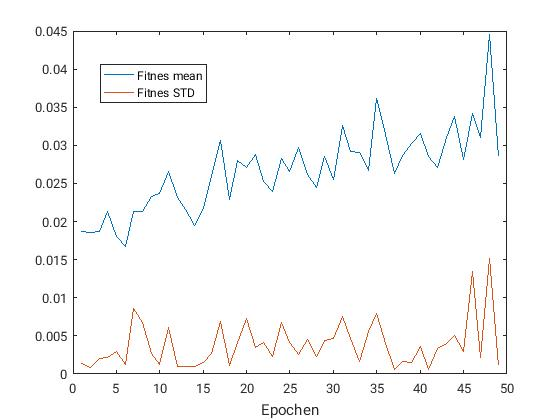
\includegraphics[width=.8\textwidth]{increasedEpochs.jpg}
}

\section{Testfallvergleich}
\frame{\frametitle{Äquivalenzklassen}
Generierte Testfall-Klassen:
\begin{figure}\centering
\subfigure{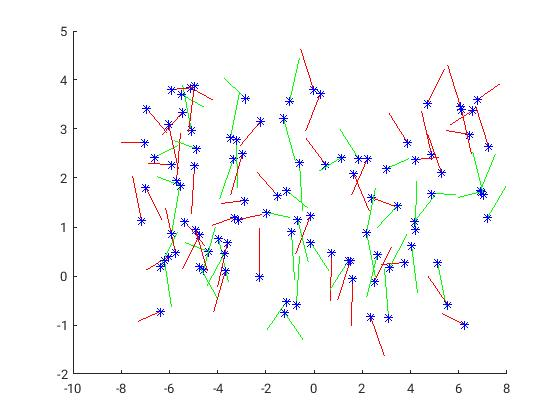
\includegraphics[width=.48\textwidth]{initialTCs.jpg}}
\subfigure{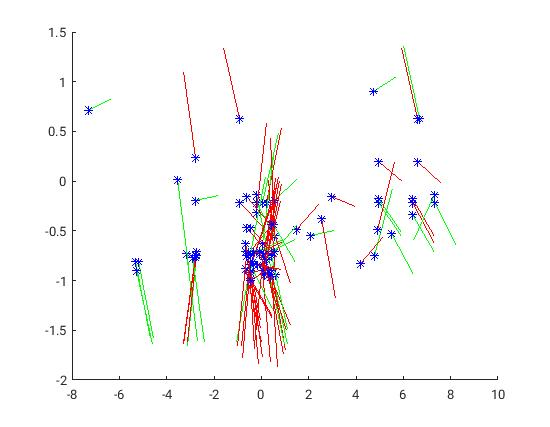
\includegraphics[width=.48\textwidth]{testcases_100chr_500epochs.jpg}}
Testfälle (Initial und nach 500 Generationen)
\end{figure}
}

\frame{\frametitle{Äquivalenzklassen}
\begin{tabular}{l|ll|ll}
& \multicolumn{2}{c}{50 Generationen} & \multicolumn{2}{c}{500 Generationen} \\
& Mittelwert & Abweichung & Mittelwert & Abweichung \\\hline
X-Position & 0.515882 & 2.301561 & 0.352941&	2.883735\\
Y-Position & 0.888431 & 0.934355  & -0.538824&	0.420933\\
Orientation & 2.456849 & 2.272890 &  3.691803&	2.331866\\
Slot-Length & 2.402382 & 0.164123 & 2.308667	&0.092787\\
Slot-Depth & 1.158000& 0.125341 & 1.116588	&0.148013
\end{tabular}

\bigskip\bigskip
Tendenz zu zentralisierter Fahrzeugposition bei kleiner Parklücke
}

\frame{\frametitle{Manuell gewählte Testfälle}
\centering
\begin{tabular}{l|l|l|l|l}
Position & Winkel & Parklücke & Fitness & Reale Eignung \\\hline
5/0 & 0 & 2.5/1 & 0.0 & Kollision \\
-5/0 & 0 & 2.5/1 & 0.0 & Kollision \\
4/0 & 0 & 2.5/1 & 0.039828 & Beinahe Kollision \\
-4/0 & 0 & 2.5/1 & 0.039828 & Beinahe Kollision \\
2/0 & 270 & 2.5/1 & 0.0 & Kollision \\
2.5/0 & 180 & 5/2 & 0.0 & Falsches Ziel und Kollision \\
-2.5/0 & 180 & 5/2 & 0.008106 & Falsches Ziel \\
0/4 &  0 & 2.5/1 & 0.020079 & Merkwürdige Fahrspur \\
0/0 &  0 & 5/2 & 0.006673 & Merkwürdige Fahrspur \\
\end{tabular}
}

\frame{\frametitle{Manuell gewählte Testfälle}
\centering
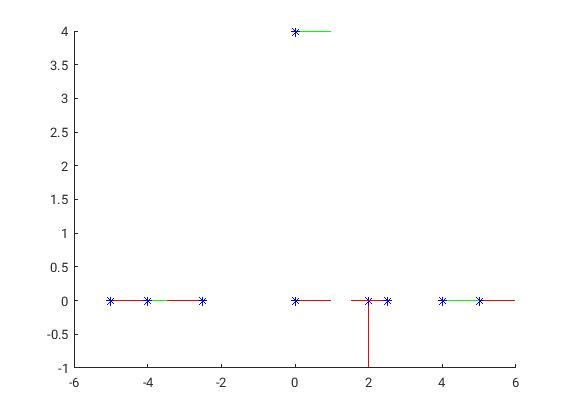
\includegraphics[width=.8\textwidth]{myTestcases.jpg}
}


\section{Ausblick}
\frame{\frametitle{Ausblick}
Zusammenfassend lässt sich sagen:
\begin{itemize}
\item Die Fitness nimmt über die Generationen zu
\item Der Algorithmus liefert bevorzugt zentrale Parkszenarien
\item Manuell abgeleitete Testfälle sind heterogener
\end{itemize}
Zukünftige Aufgaben könnten beinhalten:
\begin{itemize}
\item Formulieren eines automatisierten Abbruchkriteriums
\item Weitere Fitnessfunktionen für andere Testfall-Klassen und erhöhte Heterogenität
\item Modifikation der Konvergenz-Geschwindigkeit durch Greedy-Ansatz
\end{itemize}
}

\end{document}